\ifx\wholebook\relax\else
\input{../Common.tex}
\input{../macroes.tex}
\begin{document}
\fi


\chapter{Parameters and Arguments}\label{ch:argumenting}

\begin{chapterfigure}
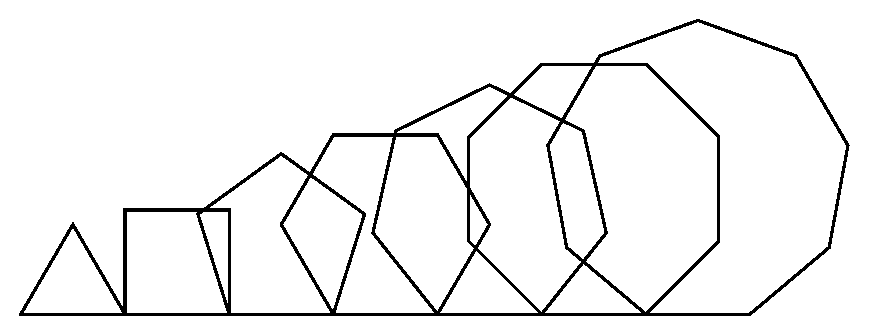
\includegraphics[width=0.9\linewidth]{ArgumentTitle}
\end{chapterfigure}

\newcommand{\replace}[2]{Up until now}{In many previous scripts} you sent messages with \emph{arguments}. For example\newcommand{\remove}[1]{,} in the message \ct{go: 100} you specified that a robot should move a distance of 100 pixels\newcommand{\add}[1]{,} and 100 is the argument of this message. You learned how to define methods but not how to define methods that require arguments. \newcommand{\add}[1]{\paragraph
}
In this Chapter, you \newcommand{\replace}[2]{shall}{will} learn how to define methods whose behavior can be parameterized. Method parameters act as holes in the method definitions, holes that are filled when the message is sent.  First we will define a method with a parameter and invoke it, then we will analyze it.

%%%%%%%%%%%%%%%%%%%%%%%%%%%%%%%%%%%%%%%%%%%%%%%

\section{Parameter, you say?!}
The method \ct{square} defined in Chapter~\ref{mth:square} is
rather limited because the size of the square is fixed once \newcommand{\add}[1]{and} for all. You \newcommand{\replace}[2]{certainly}{probably} asked yourself what should be done to draw a square \newcommand{\remove}[1]{of} 300 pixels \newcommand{\replace}[2]{or,}{wide, or} 175, or 225 or even 23 pixels\newcommand{\add}[1]{ wide}.  There is nothing preventing you \newcommand{\replace}[2]{to define}{from defining} the methods \ct{square300}, \ct{square175}, \ct{square225}, \ct{square23} and so on. \newcommand{\add}[1]{\paragraph
}
But if we \newcommand{\replace}[2]{really look at}{think about} it, creating multiple square methods does not solve the problem we have here. \newcommand{\replace}[2]{Because we do not want to}{We would rather not} define a new method each time. We would like to be able to specify the size of the square without having to define \newcommand{\remove}[1]{each time} a new method\newcommand{\add}[1]{ for every size}!
For example, we would like to be able to draw squares whose size is given by a user\newcommand{\replace}[2]{ and for}{. For} that we \newcommand{\replace}[2]{do not}{wouldn't} want to define a method.

What we need is a kind of variable whose value will be assigned when the message \newcommand{\replace}[2]{will be}{is} sent\newcommand{\add}[1]{,} and not before. This kind of \newcommand{\replace}[2]{variables exist}{variable exists} in \newcommand{\add}[1]{many} programming languages and \newcommand{\replace}[2]{are}{is} called \newcommand{\add}[1]{a} \emph{parameter}. A method parameter is a special variable which can take any value we like \emph{at the moment the message is sent}, \newcommand{\remove}[1]{and} not when we defined the method.

Come to think of it, this sounds familiar, doesn't it? After all, you know that methods such as \go or \turnLeft take a value (a distance or an angle) at the time the message is sent. All we have to do now is to understand how \newcommand{\replace}[2]{do we}{to} declare a method able to take arguments at execution time, \newcommand{\remove}[1]{just} like the method \go\newcommand{\add}[1]{ can}.

\subsection{The method \ct{square:}}
We have seen that, in \st, the name of a method is terminated by a colon (\ct{:}) to indicate that the method requires an argument. \newcommand{\replace}[2]{Thus,}{So} if we want to create a method to draw a square with an arbitrary size, we will use \ct{square:} as \newcommand{\add}[1]{its} name. We define the method \ct{square:} as shown in \methodref{mth:squareArguments}\newcommand{\add}[1]{. }
This method is then \newcommand{\replace}[2]{invoked}{used} in \newcommand{\remove}[1]{the} \scriptref{scr:usesquare}.

\begin{method}\label{mth:squareArguments}
square: \emph{size}
   "Draw a square of \newcommand{\add}[1]{the} given size"

   4 timesRepeat: 
                    [ self go: \emph{size}.
                    self turnLeft: 90 ]
\end{method}

\begin{scriptwithtitle}{Using the method \ct{square:}}\label{scr:usesquare}
| \caro |
\caro := \Turtle new.
\caro square: 10.
\caro go: 300.
\caro square: 20
\end{scriptwithtitle}

Now \newcommand{\replace}[2]{let us}{let's} analyze the method definition.  To define a method that requires one  argument, we \newcommand{\replace}[2]{terminated}{terminate} the method name with a colon \ct{:} and \newcommand{\replace}[2]{we wrote}{follow it with} the name of the parameter, \newcommand{\replace}[2]{\eg}{which is} \ct{size} in~\methodref{mth:squareArguments}. \newcommand{\add}[1]{\paragraph
}
The parameter just represents a variable whose value is defined when the message is sent \newcommand{\replace}[2]{and }{(}not when the method is defined\newcommand{\add}[1]{)}. In the script~\ref{scr:usesquare}, \newcommand{\remove}[1]{\ct{size} will take the value 10} during the first message \ct{square:\ 10} \newcommand{\replace}[2]{and then 20}{\ct{size} will have the value 10. Then} during the message \ct{square:\ 20}\newcommand{\add}[1]{, \ct{size} will have the value 20}.  The argument, however, does not need to be explicitly declared using vertical bars \ct{|} and \ct{|}.
 
In the method~\ref{mth:squareArguments} the name of the parameter is \ct{size}. The name of the parameter should represent what it is used for. Note that we could have named this parameter \ct{length} as in method~\ref{mth:squareArgumentslength}, or \ct{distance} \newcommand{\add}[1]{---} as \newcommand{\replace}[2]{soon}{long} as we replace \newcommand{\remove}[1]{in the method body} all the \newcommand{\replace}[2]{occurences}{occurrences} of \ct{size} \newcommand{\replace}[2]{by}{in the method body with} \ct{length}. Note that  \newcommand{\remove}[1]{thes} method~\ref{mth:squareArgumentslength} and  method~\ref{mth:squareArguments} \newcommand{\replace}[2]{are}{give} \emph{exactly} the same\newcommand{\add}[1]{ results}.

\begin{method}\label{mth:squareArgumentslength}
square: \emph{length}
   "Draw a square of \newcommand{\add}[1]{the} given size"

   4 timesRepeat: 
                    [ self go: \emph{length}.
                    self turnLeft: 90]
\end{method}


\section{Practicing}
Now this is time to practice a bit. \newcommand{\replace}[2]{Let us}{Let's} start with a simple exercise.

\begin{exofigwithsizeandtitle}[0.5]{\includegraphics[width=6cm]{ArgHexagon}}{\ct{hexagon:}}
  Define the method \ct{hexagon:} that draws \newcommand{\replace}[2]{an}{a} hexagon with \newcommand{\replace}[2]{side of a given size}{sides of the specified length}.
\end{exofigwithsizeandtitle}

\begin{exofigwithsizeandtitle}[0.5]{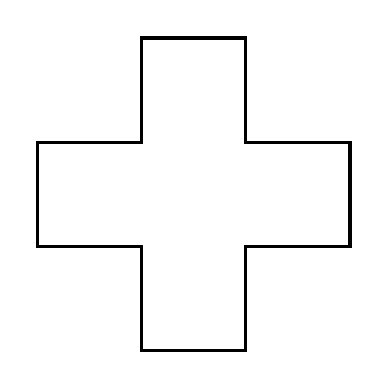
\includegraphics{Argcrossscr}}{Cross}
Transform the script given \newcommand{\replace}[2]{hereafter}{below} into a method named \ct{cross:} that draws a cross of \newcommand{\replace}[2]{a}{the} given size. You should then be able to execute the \newcommand{\remove}[1]{following} expression: \ct{\caro\ cross:\ 100}. Hint: notice that 100/ 2 = 50.
\begin{nalltt}
|\caro|
\caro := \Turtle new.
4 timesRepeat: 
               [ \caro go: 50. 
               \caro turnLeft: 90. 
               \caro go: 100. 
               \caro turnRight: 90. 
               \caro go: 100.
               \caro turnRight: 90.
               \caro go: 50 ]

\end{nalltt}
\end{exofigwithsizeandtitle}


\largecadre{To define a method with multiple \newcommand{\remove}[1]{number of} arguments\newcommand{\add}[1]{,} terminate \newcommand{\replace}[2]{the words that compose}{each word in} the method name \newcommand{\replace}[2]{by a colon}{with a colon,} and place \newcommand{\replace}[2]{between them the parameters}{each parameter after its corresponding word in the method name}.\\
The method named \ct{polygon:size:} requires two arguments. The definition of the method \ct{polygon: \newcommand{\replace}[2]{sizeNumber}{numberOfSides} size: size} defines two arguments\newcommand{\add}[1]{,} \ct{\newcommand{\replace}[2]{sizeNumber}{numberOfSides}} and \ct{size}.}

%%%%%%%%%%%%%%%%%%%%%%%%%%%%%%%%%%%%%%%%%%%%%%%
\section{Multiple Arguments}
Of course, it would be \newcommand{\replace}[2]{best}{better} to have a method drawing a polygon \newcommand{\replace}[2]{of}{with a} given number of sides
\emph{and} size. The \newcommand{\replace}[2]{problem}{question} is how \newcommand{\replace}[2]{to}{do we} create a method having two arguments\newcommand{\replace}[2]{?Creating}{?  We can create} a method with two arguments \newcommand{\remove}[1]{is obtained} by writing a method name with two colons and placing \newcommand{\replace}[2]{the}{one} argument \newcommand{\replace}[2]{names}{name} after each colon.
\newcommand{\replace}[2]{Thus,}{So} in our \newcommand{\replace}[2]{case}{example} the method is called \ct{polygon:size:}. Its code is shown below. We can then simply send the message \ct{\caro\ polygon:\ 7\ size:\ 100}.

\begin{method}\label{mth:fixedSizePolygon}
polygon: \newcommand{\replace}[2]{sideNumber}{numberOfSides} size: size
    "Draws a polygon \newcommand{\replace}[2]{of}{with the} given number of sides and size"

    | angle length |
    angle := 360 / \newcommand{\replace}[2]{sideNumber}{numberOfSides}.
    length := 4 * size / \newcommand{\replace}[2]{sideNumber}{numberOfSides}.
    sideNumber timesRepeat: 
                               [ self go: length.
                               self turnLeft: angle ]
\end{method}



\paragraph{Implementation Remark.} You may wonder why we defined \newcommand{\add}[1]{the} length as \ct{4 * size / \newcommand{\replace}[2]{sideNumber}{numberOfSides}}. We decided to make the \newcommand{\replace}[2]{polygon'}{polygon's} perimeter \newcommand{\replace}[2]{equals}{equal} to the \newcommand{\replace}[2]{one}{perimeter} of a
square \newcommand{\replace}[2]{having}{that has} a side of \newcommand{\remove}[1]{size} length\newcommand{\add}[1]{ \ct{size}}. This way the perimeter is constant \newcommand{\add}[1]{regardless of the \ct{numberOfSides},} and all the polygons will be displayed using \newcommand{\add}[1]{about} the same \newcommand{\replace}[2]{part}{fraction} of the screen. 

Here is the code of the method \ct{polygon100:} which draws a polygon \newcommand{\replace}[2]{of a}{with the} given number of sides\newcommand{\add}[1]{, each side} having a length of 100 pixels.

\begin{method}\label{mth:regularPolygon}
polygon100: \newcommand{\replace}[2]{sideNumber}{numberOfSides}
    "Draws a polygon \newcommand{\replace}[2]{of}{with the} given number of sides\newcommand{\replace}[2]{,}{;} the \newcommand{\replace}[2]{size}{length} of each
    side is 100 pixels"

    | angle |
    angle := 360 / \newcommand{\replace}[2]{sideNumber}{numberOfSides}.
    sideNumber timesRepeat: 
                               [ self go: 100.
                               self turnLeft: angle ]
\end{method}

This method has one argument, \ct{\newcommand{\replace}[2]{sideNumber}{numberOfSides}}, and one variable, \ct{angle}. Both of them are used within the code of the method. \newcommand{\replace}[2]{\ct{sideNumber}}{\ct{numberOfSides}'s} value is specified by \newcommand{\replace}[2]{a}{the} message that uses the method\newcommand{\add}[1]{,} for example \ct{\caro\ polygon100:\ 7}\newcommand{\replace}[2]{, while the}{. The} variable \ct{angle} is initialized by computing the angle corresponding to the parameter values (\newcommand{\replace}[2]{here}{namely} 360 / 7\newcommand{\add}[1]{ in our example}). For \newcommand{\replace}[2]{each}{any} value of \newcommand{\replace}[2]{the \ct{sideNumber}}{\ct{numberOfSides}}, \ct{angle} will \newcommand{\replace}[2]{then take a specific}{get the right} value\newcommand{\add}[1]{ for the polygon}.

\begin{scriptfig}{Arghepta}{Using the method \ct{polygon100:}}\label{src:heptagon}
| \caro |
\caro := \Turtle new.
\caro polygon100: 7.
\end{scriptfig}

You may think that the name of the parameter \ct{\newcommand{\replace}[2]{sideNumber}{numberOfSides}} is long. However, this name can easily be understood by any person reading the method. As we already discussed in Chapter~\ref{ch:furthervariables}, it is quite important that anyone be able \newcommand{\add}[1]{to} read your code\newcommand{\replace}[2]{,}{---} almost like a \newcommand{\replace}[2]{novel}{story}. 


@@dank: The crossWidth:height: exercise and figures are more convoluted and obscure than necessary for beginners' practice with two arguments.  I expect many students would give up in discouragement.  I recommend substituting a straightforward example such as rectangleWidth:height:. If you keep this exercise, I strongly recommend adding a decomposed or 'exploded' diagram of a cross, with labeled or colored segments showing what each parameter controls. More explanatory parameter names would also help. @@
\begin{exonofig}
By slightly modifying the method \ct{cross:}, define the method
\ct{crossWidth:height:} that \newcommand{\replace}[2]{allows you to}{can} draw the \newcommand{\replace}[2]{picture}{crosses} shown in
Figure~\ref{fig:c8croix1}.  Note that a normal cross corresponds to
\ct{caro crossWidth: 30 height: 60}
\end{exonofig}


\begin{figure}[!h]
\begin{minipage}[c]{.3\linewidth}
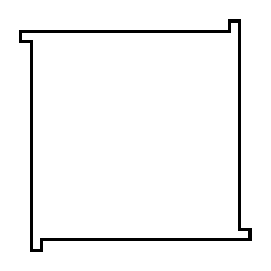
\includegraphics{Argcrossscr2.pdf}
\end{minipage}
\begin{minipage}[c]{.3\linewidth}
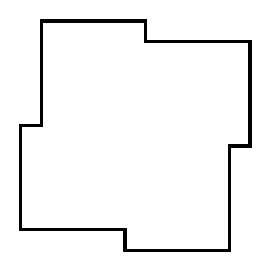
\includegraphics{Argcrossscr3}
\end{minipage}
\begin{minipage}[c]{.3\linewidth}

\includegraphics[width=5cm]{Argcrossscr4}
\end{minipage}
\label{c8croix1}
\caption{Three crosses \newcommand{\replace}[2]{produces respectively by:}{produced by \ct{crossWidth:height:} messages. The cross on the left is from} \ct{\caro crossWidth: 5 height: 50}\newcommand{\replace}[2]{,}{; in the middle, from} \ct{\caro crossWidth: 50 height: 5}\newcommand{\replace}[2]{ and}{; on the right, from} \ct{\caro crossWidth: 10 height: 20} \label{fig:c8croix1}\newcommand{\add}[1]{.}}
\end{figure}




%%%%%%%%%%%%%%%%%%%%%%%%%%%%%%%%%%%%%%%%%%%%%%%
\section{Parameters and Variables}
Now that \newcommand{\replace}[2]{you}{you've} practiced a bit, it is time to look \newcommand{\remove}[1]{a bit} more carefully at the difference between variables and parameters. \newcommand{\replace}[2]{For this purpose let us}{Let's} compare \newcommand{\remove}[1]{the} \scriptref{scr:Argsquarewithvariable} and \newcommand{\remove}[1]{the method} \methodref{mth:squareArgumentsagain} \newcommand{\add}[1]{that we} defined earlier \newcommand{\replace}[2]{that we repeat here}{(see copies below)}. 

\newcommand{\replace}[2]{From the}{In} \scriptref{scr:Argsquarewithvariable} \newcommand{\replace}[2]{we see that:  First}{first} the variable \ct{size} is declared (line 1), then \newcommand{\remove}[1]{assign it} a value \newcommand{\add}[1]{is assigned to it} (line 3) and \newcommand{\replace}[2]{then}{finally} it is used as \newcommand{\add}[1]{the} argument of the method \go (line 5).

\begin{scriptwithtitle}{The square script using a variable}\label{scr:Argsquarewithvariable}
(1)   | \caro \bold{size} | 
(2)   \caro := \Turtle new.
(3)   \bold{size := 10.}
(4)   4 timesRepeat: 
(5)               [ \caro go: \bold{size}.
(6)               \caro turnLeft: 90 ]
\end{scriptwithtitle}

\newcommand{\replace}[2]{Looking at}{In} \mthref{mth:squareArgumentsagain} we see \newcommand{\replace}[2]{that:}{examples of two features of parameters.}
First\newcommand{\add}[1]{,} the parameter \ct{size} is declared because it appears after
a colon in the method name (line 1). Second, it is used
as \newcommand{\add}[1]{the} parameter of the message \go (line 5). A parameter does not have to be initialized because it always gets the value specified \newcommand{\replace}[2]{by}{in} the message that uses the method.

\begin{method}\label{mth:squareArgumentsagain}
(1) square: \bold{size}
(2)   "Draw a square of \newcommand{\add}[1]{the} given size"
(3)
(4)   4 timesRepeat: 
(5)                    [ self go: \bold{size}.
(6)                    self turnLeft: 90]
\end{method}
@@dank: I found the order of presentation in the next section confusing.  I've suggested a reorganization for your consideration.@@
\paragraph{Some Other Differences.}
\newcommand{\replace}[2]{Apart from the fact that a parameter is declared within the method's name, and not using variable declaration vertical bars \ct{||}, a parameter is used in the code of the method like any other variables.}{Unlike other variables, a parameter doesn't have a variable declaration between vertical bars \ct{||}.  A parameter is declared when it appears after a colon \ct{:} in the first line of the method's definition. \paragraph
} 
\newcommand{\replace}[2]{One difference that is specific to \st is that parameters are variables that}{Another difference is that parameters} cannot be modified\newcommand{\add}[1]{ the way other variables can}. We cannot assign new values to parameters inside method bodies.\newcommand{\add}[1]{\paragraph
}
The other difference is the way values are assigned to variables and parameters. A variable value is changed using \ct{:=}.  A parameter value is initialized when the method is executed. For example, \ct{\caro\ square:\ 10} initializes the parameter \ct{size} with the value \ct{10}. A parameter is a variable. However, the  parameter's value is only known when a message is sent and the method executed.
\newcommand{\add}[1]{\paragraph
Besides those three differences, a parameter is used in the code of the method like any other variable.}
@@dank: Move this figure to follow the paragraph that refers to it in the next section?@@
\begin{figure}[h]
\begin{center}
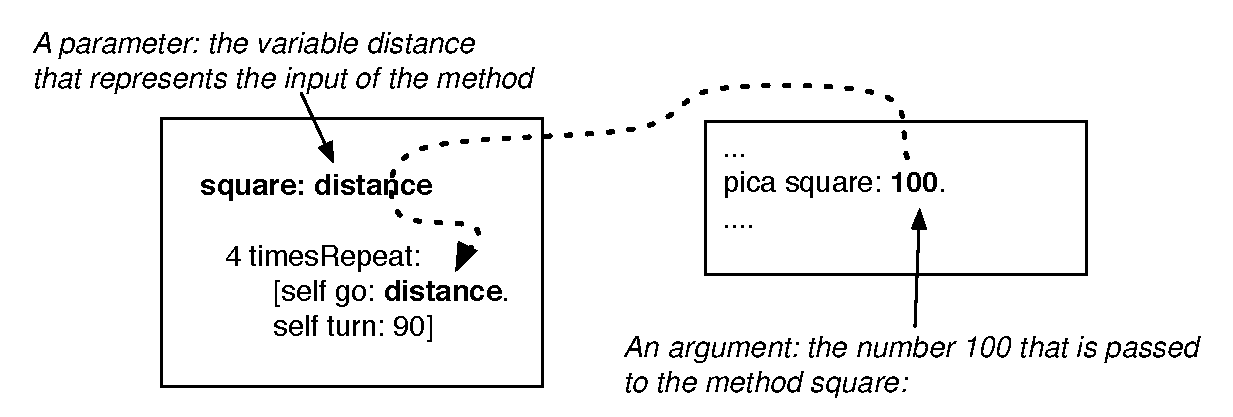
\includegraphics[width=10cm]{argparam2}
\caption{\newcommand{\replace}[2]{Difference}{The connection} between \newcommand{\replace}[2]{arguments (objects)}{an argument (an object)} and \newcommand{\replace}[2]{parameters (variables)}{a parameter (a variable)}.\label{fig:argparam}}
\end{center}
\end{figure}

\section{Arguments and Parameters} 
We use the two terms \emph{arguments} and \emph{parameters}\newcommand{\add}[1]{ for related but different ideas}.  An argument is the \newcommand{\replace}[2]{actual}{specific} object passed in a message\newcommand{\replace}[2]{, while a}{. A} parameter is the variable used in \newcommand{\replace}[2]{the}{a} method definition\newcommand{\add}[1]{, whose precise value isn't known when the method is defined}\footnote{\newcommand{\replace}[2]{Other authors call argument actual parameters and parameters formal parameters, others use parameter and argument interchangeably.}{Many authors define these terms differently. Some use "actual parameters" for what we call "arguments", and "formal parameters" for what we call "parameters". Others use the terms "parameter" and "argument" interchangeably.}}. \newcommand{\add}[1]{\paragraph
}
In Figure~\ref{fig:argparam}, in the message \ct{square: 100}, the number \ct{100} is the message argument. When the method \ct{square:} is executed its parameter \ct{distance} is initialized to \ct{100}, the value of the argument. \newcommand{\add}[1]{\paragraph
}
Another way to understand the difference between an argument and a parameter is that a parameter \newcommand{\add}[1]{is} a variable inside a method \newcommand{\replace}[2]{representing}{that represents} an input\newcommand{\add}[1]{ to the method}, while an argument is the actual value we pass to this input. \newcommand{\add}[1]{\paragraph
}
Note that a parameter can also be used as an argument \newcommand{\replace}[2]{to}{in} other message sends. For example in the definition of the method \ct{square:} (method~\ref{mth:squareArguments}), the parameter \ct{size} is used as \newcommand{\add}[1]{the} argument in the message \ct{go: size}.



A message argument can \newcommand{\replace}[2]{be also}{also be} a variable. For example in \scrref{scr:varasArg}, the argument of the first message \ct{square:} is the value of the variable \ct{dist}, \newcommand{\replace}[2]{\ie}{i.e.} 100. The argument of the second message \ct{square:} is the value of the expression \ct{dist + 200}\newcommand{\replace}[2]{ \ie}{, i.e.} 300. The parameter \ct{size} of the method \ct{square:} \newcommand{\replace}[2]{will then takes}{gets} the value \ct{100} \newcommand{\replace}[2]{for}{from} the first message\newcommand{\add}[1]{,} and then the value \ct{300} \newcommand{\replace}[2]{for}{from} the last message\newcommand{\remove}[1]{ send}. 

\begin{scriptwithtitle}{A variable as argument}\label{scr:varasArg}
| \caro dist |
\caro := \Turtle new.
dist := 100. 
\caro square: dist.
\caro go: 300.
\caro square: dist + 200
\end{scriptwithtitle}

@@dank: Move this figure to follow the paragraph that refers to it in the next section?@@
\begin{figure}[h]
\begin{center}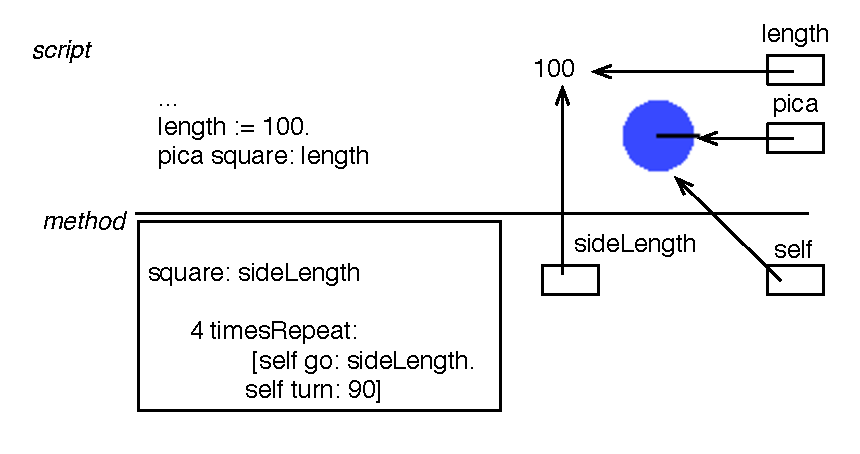
\includegraphics[width=8cm]{argumentBoxes}\end{center}
\caption{When a method is executed\newcommand{\add}[1]{,} new variables are created that refer to the arguments and the receiver. \label{fig:argumentswithboxes}}
\end{figure}


\paragraph{About Method Execution.}
\newcommand{\replace}[2]{In fact when}{When} a method is executed new variables are created. These variables are the message receiver (\ct{\newcommand{\replace}[2]{self)}{self}}) and the parameters of the method that refer to the method \newcommand{\replace}[2]{argument}{arguments} (\ct{size}  in Figure~\ref{fig:argumentswithboxes}). Figure~\ref{fig:argumentswithboxes} shows the effect of sending the message \ct{square: length} to a robot referred \newcommand{\add}[1]{to} by the variable \newcommand{\replace}[2]{\ct{pica}}{\ct{\caro}}, \newcommand{\add}[1]{when} the variable \ct{length} \newcommand{\replace}[2]{referencing}{references} the number \ct{100}. When the method \ct{square:} is executed, the variable \ct{self} refers to the message receiver, \ie the robot pointed to by the variable \newcommand{\replace}[2]{\ct{pica}}{\ct{\caro}}, and the parameter \ct{size} refers to the value of the variable \ct{length}, \ie the number \ct{100}. 
The execution of the expression \ct{\daly\ square:\ 200} assigns to \self the robot referenced by the variable \daly\newcommand{\add}[1]{,} and \newcommand{\replace}[2]{\ct{200} to the value of \ct{size}}{assigns to \ct{size} the number \ct{200}}. 

This may look complex but you do not have to \newcommand{\replace}[2]{worry: Parameters are variables that}{worry about it. These are the hidden steps \st takes to make sure that parameters} are initialized with the values \newcommand{\replace}[2]{of}{in} the messages.



\summa

\begin{enumerate}
  \item A method parameter is declared right after the colon
  indicating the position of the parameter. It must not be declared as a  variable.
  
 \item To define a method with multiple \newcommand{\remove}[1]{number of} arguments\newcommand{\add}[1]{,} terminate \newcommand{\replace}[2]{the words that compose}{each word in} the method name \newcommand{\replace}[2]{by a colon}{with a colon,} and place \newcommand{\replace}[2]{between them the parameters}{each parameter after its corresponding word in the method name}.\\
The method named \ct{polygon:size:} requires two arguments. The definition of the method \ct{polygon: \newcommand{\replace}[2]{sizeNumber}{numberOfSides} size: size} defines two arguments\newcommand{\add}[1]{,} \ct{\newcommand{\replace}[2]{sizeNumber}{numberOfSides}} and \ct{size}.\end{enumerate}


\ifx\wholebook\relax\else\end{document}\fi
